\documentclass{gadsescript}

\setsemester{Winter Semester 2023/2024}%
\setuniversity{University of Konstanz}%
\setfaculty{Faculty of Science\\(Mathematics and Statistics)}%
\settitle{BMA}

\newcommand{\farbe}{%
	{\color{gadse-red}f}%
	{\color{gadse-orange}a}%
	{\color{gadse-dark-blue}r}%
	{\color{gadse-dark-green}b}%
	{\color{gadse-pink}e}%
}
\newcommand{\rot}{{\color{gadse-red}rot}}
\newcommand{\gruen}{{\color{gadse-dark-green}gruen}}
\newcommand{\blau}{{\color{gadse-dark-blue}blau}}
\newcommand{\bunt}{{\color{gadse-pink}bunt}}

\newcommand{\staerkerot}{{\color{gadse-red}staerke_{rot}}}
\newcommand{\staerkegruen}{{\color{gadse-dark-green}staerke_{gruen}}}
\newcommand{\staerkeblau}{{\color{gadse-dark-blue}staerke_{blau}}}
\newcommand{\staerkebunt}{{\color{gadse-pink}staerke_{bunt}}}

\begin{document}
\maketitle
\begin{enumerate}[label=(\alph*)]
	\item Wir nehmen die Standardbasis von $ \R^3 $ und lassen
		\[
			 f: \R^3 \to \R^3,
			 \begin{pmatrix} 1\\0\\0\\ \end{pmatrix} \mapsto \begin{pmatrix} 1\\2\\3\\ \end{pmatrix},
			 \begin{pmatrix} 0\\1\\0\\ \end{pmatrix} \mapsto \begin{pmatrix} 4\\5\\6\\ \end{pmatrix},
			 \begin{pmatrix} 0\\0\\1\\ \end{pmatrix} \mapsto \begin{pmatrix} 0\\0\\0\\ \end{pmatrix}.
		\]
		\textbf{Beh.:} $ f(\R^3) = \Span \left\{ \begin{pmatrix} 1\\2\\3\\ \end{pmatrix}, \begin{pmatrix} 4\\5\\6\\ \end{pmatrix}   \right\}  $ 
	\item \textbf{Vor.:}
		Seien 
		\[ \color{gadse-red} rot \coloneqq \begin{pmatrix} 1\\0\\0\\0\\ \end{pmatrix}, \]
		\[ \color{gadse-dark-green} gruen \coloneqq v_1, \]
		\[ \color{gadse-dark-blue} blau \coloneqq v_2, \]
		\[ \color{gadse-pink} bunt \coloneqq \begin{pmatrix} 0\\0\\0\\1\\ \end{pmatrix}, \]
		\textbf{Beh.:} $ \left\{ \rot, \gruen, \blau, \bunt \right\}  $ eine Basis von $ \R ^4 $ und für
		\[
			\farbe: \R ^4 \to \R ^3, \rot \mapsto e_1, \gruen \mapsto 0, \blau \mapsto 0, \bunt \mapsto e_2
		\]
		gilt
		$ \Kern (\farbe) = \Span \left\{ \gruen, \blau \right\}  $
\end{enumerate}
\begin{proof*}
	\begin{enumerate}[label=(\alph*)]
		\item 
			\begin{description}
				\item[``$ \subseteq $'':] Sei $ gadse \in \R ^3 $, zu zeigen $ gadse \in \Span \left\{ v_1, v_2 \right\} $:
					Da $ gadse \in \R ^3 $ gilt $ \exists hut, stock, regenschirm \in \R : gadse = hut \cdot e_1 + stock \cdot e_2 + regenschirm \cdot e_3 $. Dann gilt:
					\begin{align*}
						f(gadse) &= f(hut \cdot e_1 + stock \cdot e_2 + regenschirm \cdot e_3 \\
						~&= hut \cdot f(e_1) + stock \cdot f(e_2) + regenschirm \cdot f(e_3) \\
						~&= hut \cdot v_1 + stock \cdot v_2 \in \Span \left\{ v_1, v_2 \right\}  \\
					\end{align*}
				\item[``$ \supseteq $'':] Sei $ gadse \in \Span \left\{ v_1, v_2 \right\}  $, zu zeigen $ \exists urgadse \in \R ^3 : f(urgadse) = gadse $:
					Da $ gadse \in \Span \left\{ v_1, v_2 \right\} : \exists hut, stock \in \R ^3 : gadse = hut \cdot v_1 + stock \cdot v_2 $.
					Setze $ urgadse \coloneqq hut \cdot e_1 + stock \cdot e_2 $, sodass
					\begin{align*}
						f(urgadse) &= f(hut \cdot e_1 + stock \cdot e_2) \\
						~&= hut \cdot f(e_1) + stock \cdot f(e_2) \\
						~&= hut \cdot v_1 + stock \cdot v_2 \\
						~&= gadse \qed
					\end{align*}
			\end{description}
		\item 
			Um zu zeigen, dass $ \left\{ \rot, \gruen, \blau, \bunt \right\} $ eine Basis von $ \R ^4 $ reicht zu zeigen,
			dass $ \left| \left\{ \rot, \gruen, \blau, \bunt \right\} \right| = \Dim \R ^4 $ und $ e_1, e_2, e_3, e_4 \in \Span \left\{ \rot, \gruen, \blau, \bunt \right\} $.
			$ \left| \left\{ \rot, \gruen, \blau, \bunt \right\} \right| = 4 =  \Dim \R ^4 $ trivialer Weise. Und 
			\[ e_1 = \rot \]
			\[ e_2 = \gruen - \rot - \blau - 2 \cdot \bunt \]
			\[ e_3 = \gruen - \rot - 2 \cdot \blau - \bunt \]
			\[ e_4 = \bunt \]
			\begin{description}
				\item[``$ \subseteq $''] Sei $ gadse \in \Kern (\farbe) $, sodass $ \farbe(gadse) = 0 $, es gilt zu zeigen $ gadse \in \Span(\gruen, \blau) $.\\
					Angenommen $ gadse \centernot\in \Span \left\{ \gruen, \blau \right\}  $,
					dann gilt
					\[ \exists \staerkerot, \staerkegruen, \staerkeblau, \staerkebunt \in \R \text{, für die gilt} \]
					\[ \staerkerot \neq 0 \vee \staerkebunt \neq 0 \text{ und} \] 
					\[ gadse = \staerkerot \cdot \rot + \staerkegruen \cdot \gruen + \staerkeblau \cdot \blau + \staerkebunt \cdot \bunt \text{, dann gilt} \]
					\begin{align*}
						\farbe(gadse) &= \farbe( \staerkerot \cdot \rot + \staerkegruen \cdot \gruen\\
						~&\qquad + \staerkeblau \cdot \blau + \staerkebunt \cdot \bunt) \\
						~&= \staerkerot \cdot \farbe(\rot) + \staerkegruen \cdot \farbe(\gruen) \\
						~&\qquad + \staerkeblau \cdot \farbe(\blau) + \staerkebunt \cdot \farbe(\bunt) \\
						~&= \staerkerot \cdot e_1 + \staerkebunt \cdot e_2 \\
					\end{align*}
					und da $ e_1, e_2 $ linear unabhängig und $ \staerkerot \neq 0 \vee \staerkebunt \neq 0 $ gilt
					\[
						\farbe(gadse) \neq 0,
					\]
					was im Wiederspruch zur Annahme steht, also muss $ gadse \in \Span \left\{ \gruen, \blau \right\}  $ sein.
				\item[``$ \supseteq $''] Sei $ gadse \in \Span \left\{ \gruen, \blau \right\}  $, zu zeigen $ gadse \in \Kern (\farbe) $.\\
					Für $ gadse \in \Span \left\{ \gruen, \blau \right\}  $ gilt $ \exists \staerkegruen, \staerkeblau \in \R  $ mit $ gadse = \staerkegruen \cdot \gruen + \staerkeblau \cdot \blau $, dann gilt 
					\begin{align*}
						\farbe\left( gadse \right) &= \farbe\left( \staerkegruen \cdot \gruen + \staerkeblau \cdot \blau \right) \\
						~ &= \staerkegruen \cdot \farbe\left( \gruen \right) +\staerkeblau \farbe\left( \blau \right)  \\
						~&= 0 \\
					\end{align*}
					somit ist $ gadse \in \Kern\left( \farbe \right)  $\qed
			\end{description}
	\end{enumerate}
\end{proof*}

\begin{figure}[htpb]
	\centering
	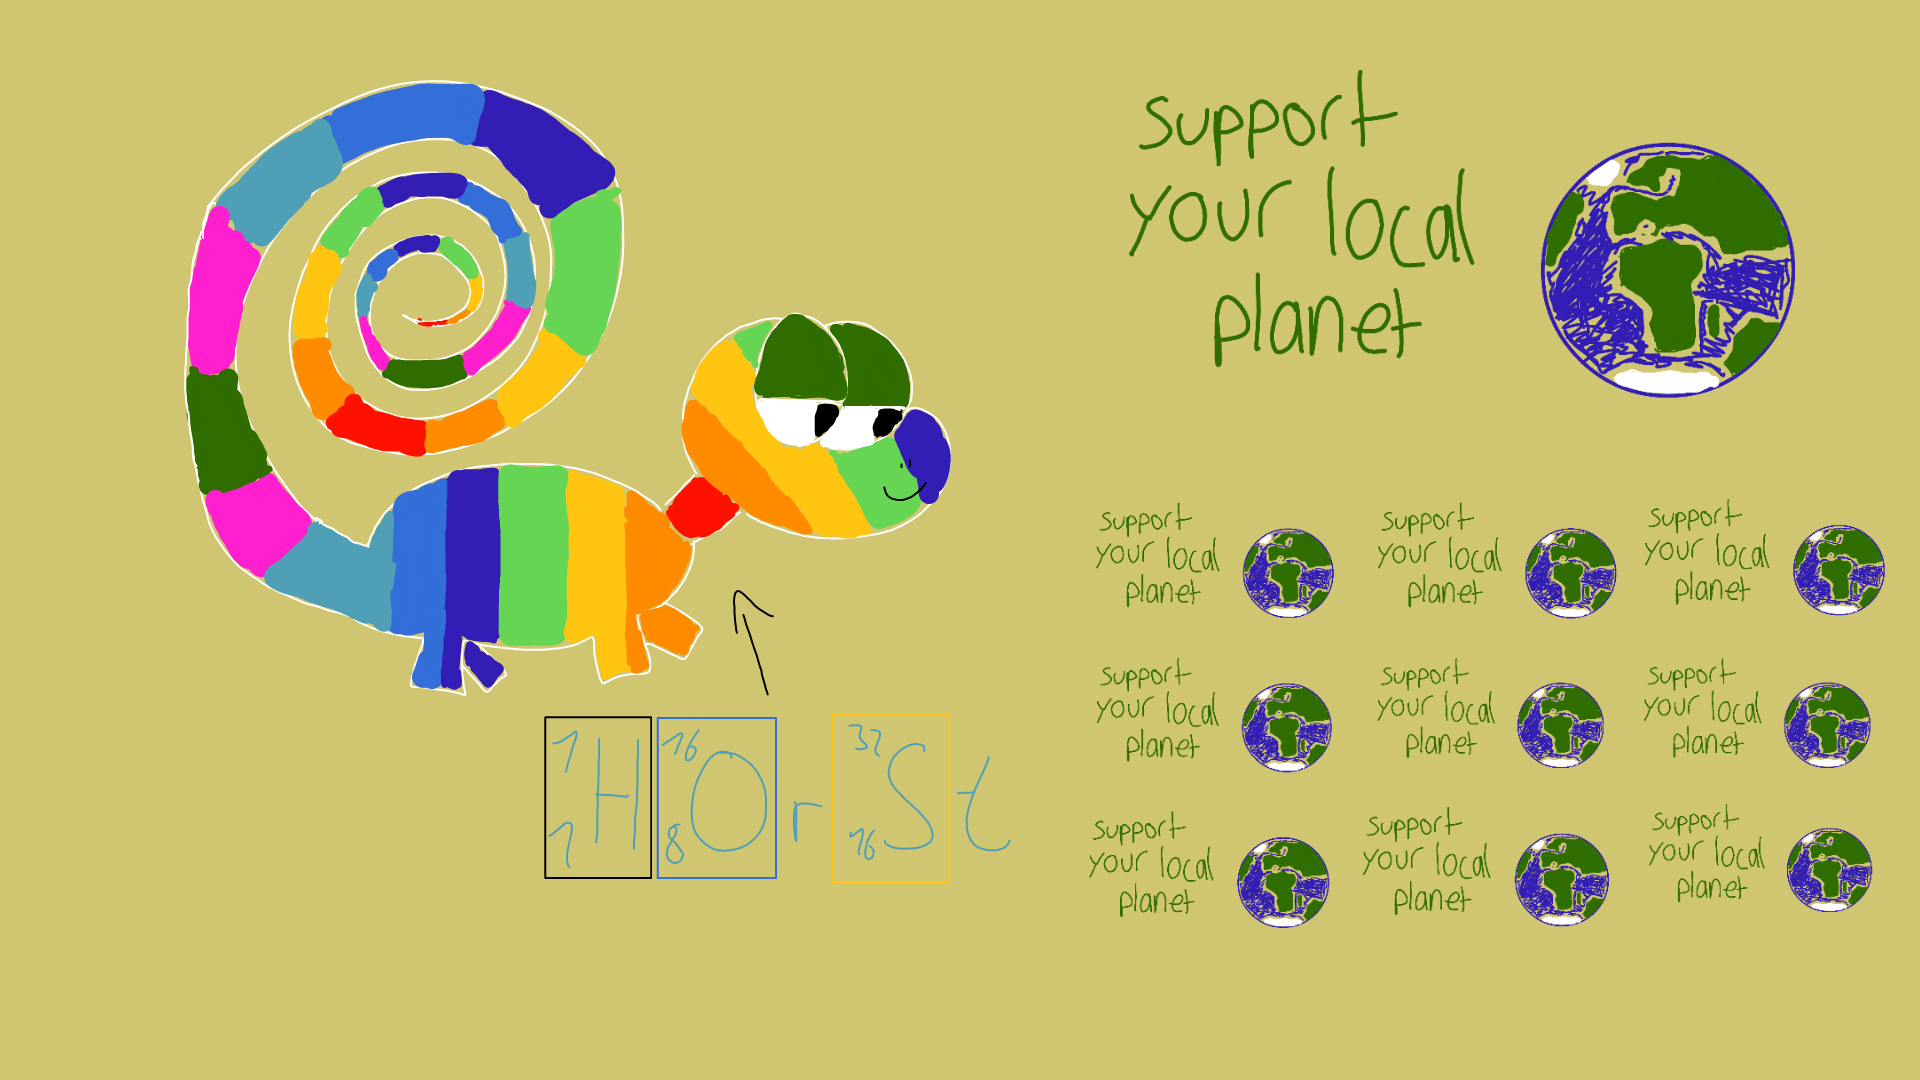
\includegraphics[width=0.8\textwidth]{1.png}
	\caption{OG gadse}
	\label{fig:gadse}
\end{figure}
\end{document}
